\documentclass{standalone}
\usepackage{tikz}
\usepackage{ctex,siunitx}
\setCJKmainfont{Noto Serif CJK SC}
\usepackage{tkz-euclide}
\usepackage{amsmath}
\usetikzlibrary{patterns, calc,3d}
\usetikzlibrary {decorations.pathmorphing,decorations.pathreplacing,decorations.shapes}
\begin{document}
\small
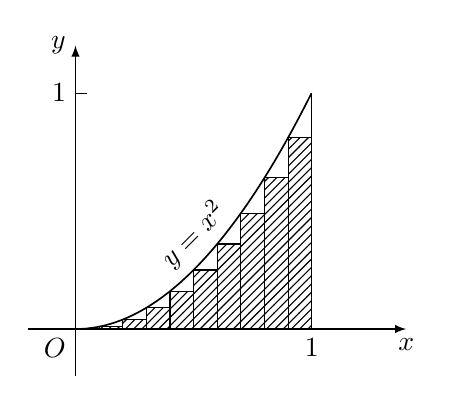
\begin{tikzpicture}[>=latex,scale=3]
  \draw[->](-0.2,0)--(1.4,0)node[below]{$x$};
  \draw[->](0,-0.2)--(0,1.2)node[left]{$y$};
  \node at (0,0)[below left]{$O$};
  \draw[semithick,samples=200,domain=0:1]plot(\x,\x*\x);
  \node at (0.5,0.4)[rotate=45]{$y=x^2$};
  \foreach \x in {1,...,9}
  {
    \draw[pattern =north east lines](0.1*\x,0)rectangle++(0.1,0.01*\x*\x);
  }
  \draw(1,1)--(1,0)node[below]{1};
  \draw[very thin](0,1)node[left]{1}--(0.05,1);
\end{tikzpicture}
\end{document}